% CVPR 2026 Paper Template; see https://github.com/cvpr-org/author-kit

\documentclass[10pt,twocolumn,letterpaper]{article}

%%%%%%%%% PAPER TYPE
\usepackage{cvpr}

% Import additional packages in the preamble file, before hyperref
\input{preamble}
\usepackage{booktabs}
\usepackage{subcaption}
\usepackage{float}

% It is strongly recommended to use hyperref, especially for the review version.
% hyperref with option pagebackref eases the reviewers' job.
% Please disable hyperref *only* if you encounter grave issues, 
% e.g. with the file validation for the camera-ready version.
%
% If you comment hyperref and then uncomment it, you should delete *.aux before re-running LaTeX.
% (Or just hit 'q' on the first LaTeX run, let it finish, and you should be clear).
\definecolor{cvprblue}{rgb}{0.21,0.49,0.74}
\usepackage[pagebackref,breaklinks,colorlinks,allcolors=cvprblue]{hyperref}

%%%%%%%%% COURSEWORK METADATA
\def\paperID{COMP6252-CW1}
\def\confName{COMP6252}
\def\confYear{2026}

%%%%%%%%% TITLE
\title{Music Genre Classification on GTZAN:
Comparative Deep Learning Baselines and Analysis}

%%%%%%%%% AUTHOR
\author{Vaishnavi Kanduri\\
University of Southampton\\
ECS User ID: \texttt{vkln25}\\
\texttt{vkln25@soton.ac.uk}
}

\begin{document}
\maketitle
\begin{abstract}
This report presents the full Part~1 implementation for music genre classification on GTZAN, following the coursework requirement to compare six neural models: Net1 (fully connected baseline), Net2 (CNN), Net3 (CNN+BatchNorm), Net4 (CNN+BatchNorm+RMSProp), Net5 (LSTM), and Net6 (LSTM with GAN-augmented training data). The workflow uses a shared stratified split (70\% train, 20\% validation, 10\% test), with spectrogram images resized to $180\times180$ and audio represented as fixed-length MFCC(+delta) sequences.

Evaluation is performed on the same held-out test set for all models with accuracy, macro precision/recall/F1, and confusion-matrix analysis. The strongest model is Net6 at 71.0\% test accuracy (macro-F1 0.7045), followed closely by Net3 at 70.0\%. The baseline progression confirms clear gains from architectural choices: Net1$\rightarrow$Net2 improves by +8.0 percentage points, and Net2$\rightarrow$Net3 by +9.0 points. Net4 (67.0\%) shows that optimizer choice can materially affect convergence quality under the same architecture, while Net5$\rightarrow$Net6 (+2.0 points) indicates a modest benefit from GAN-based augmentation.

Overall, the results show that both image-based and audio-sequence pipelines are competitive, with the final ranking led by audio models in this run. The report details implementation decisions, quantitative comparison, per-genre behavior, and practical trade-offs relevant to model selection.
\end{abstract}    
\section{Introduction}
\label{sec:intro}

This report presents Task~5.1 for music genre classification on GTZAN~\cite{tzanetakis2002gtzan}. The goal is to compare six required models under one common test split and explain the journey in simple steps: what I tried, what I got, and what I learned.

I implemented six models in PyTorch~\cite{paszke2019pytorch}: Net1 (FC), Net2 (CNN), Net3 (CNN+BatchNorm~\cite{ioffe2015batchnorm}), Net4 (CNN+BatchNorm+RMSProp), Net5 (BiLSTM~\cite{hochreiter1997lstm}), and Net6 (BiLSTM with GAN-augmented training data~\cite{goodfellow2014gan}).

The report focuses on three practical comparisons: (1) image models (Net1--Net4), (2) audio models (Net5--Net6), and (3) all six models together. I also include a student learning curve to show how performance changed as I improved the pipeline step by step.

\subsection{Main Outcome}

The best model is Net6 with 71.0\% test accuracy and 0.7045 macro-F1. The strongest image model is Net3 with 70.0\% accuracy. These results show that both image and audio pipelines are competitive, with a small final advantage for the audio-based setup in this run.

\subsection{Report Flow}

\Cref{sec:implementation} explains dataset setup, preprocessing, and architectures with in-place figures. \Cref{sec:results} is written in a simple tried $\rightarrow$ got $\rightarrow$ learned structure, with compact comparison graphs of the 4 image models, the 2 audio models, and all 6 models.

\section{Methodology}
\label{sec:implementation}

\subsection{GTZAN Dataset}

GTZAN contains 1000 clips (10 genres, 100 clips each)~\cite{tzanetakis2002gtzan}. One file (\texttt{jazz.00054.wav}) is corrupted, so the usable dataset size is 999.

I used both modalities:
\begin{itemize}
\item \textbf{Image path}: precomputed spectrogram images.
\item \textbf{Audio path}: waveform clips converted to MFCC-based sequences.
\end{itemize}

\begin{figure}[t]
	\centering
	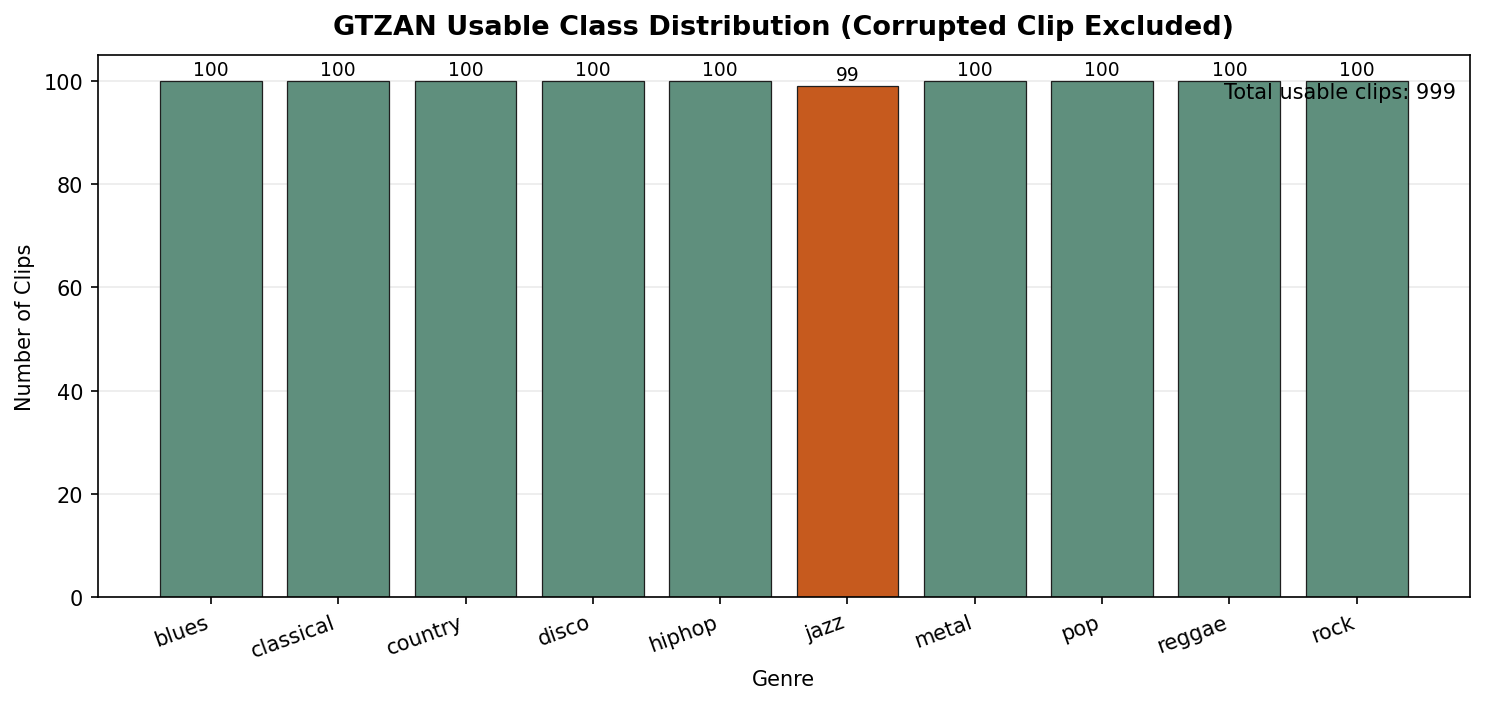
\includegraphics[width=\linewidth]{figures/gtzan_dataset_overview.png}
	\caption{GTZAN class balance and distribution used in this project (999 usable clips).}
	\label{fig:dataset-overview}
\end{figure}

\subsection{Data Split and Preprocessing}

I created one shared stratified split for every model: 70\% train, 20\% validation, 10\% test. Using one split keeps the comparison fair.

For image models (Net1--Net4), each spectrogram is resized to $180\times180$, converted to tensor, and normalized.

For audio models (Net5--Net6), each clip is resampled to 22050~Hz and converted to 80-dim features (40 MFCC + 40 delta). Sequences are padded/truncated to 320 frames.

\subsection{Neural Network Architectures}

\begin{itemize}
\item \textbf{Net1}: fully connected image baseline.
\item \textbf{Net2}: CNN baseline.
\item \textbf{Net3}: CNN + batch normalization.
\item \textbf{Net4}: Net3 architecture trained with RMSProp.
\item \textbf{Net5}: bidirectional LSTM on MFCC sequences.
\item \textbf{Net6}: Net5 with GAN-augmented training data.
\end{itemize}

\subsection{Training and Evaluation Setup}

All models are implemented in PyTorch~\cite{paszke2019pytorch}. Image models were trained up to 100 epochs with best-validation checkpoint loading. Sequence models used early stopping and gradient clipping for stable training.

Cross-entropy loss was used for classification. Adam/AdamW was used in most models, while Net4 used RMSProp by design. Net6 used weighted handling of synthetic samples during training.

The same test split was used for all six models. I report accuracy and macro-F1, then compare model groups (4 image models, 2 audio models, all 6 together) and summarize the main error pattern.
\section{Results and Discussion}
\label{sec:results}

\subsection{Quantitative Snapshot from Phase 4}

Table~\ref{tab:phase4-results} is updated from the saved outputs of \textit{Phase 4 - Evaluation and Analysis} (Task 4.1). All six models are evaluated on the same 100-sample test split.

\begin{table}[H]
	\centering
	\caption{Phase 4 overall performance summary (Task 4.1).}
	\label{tab:phase4-results}
	\scriptsize
	\setlength{\tabcolsep}{3.5pt}
	\resizebox{\columnwidth}{!}{%
	\begin{tabular}{lcccc}
		\toprule
		Model & Mod. & Epochs & Acc. (\%) & Macro-F1 \\
		\midrule
		N1 (FC) & Img & 100 & 53.0 & 0.5185 \\
		N2 (CNN) & Img & 100 & 61.0 & 0.6019 \\
		N3 (CNN+BN) & Img & 100 & 70.0 & 0.6853 \\
		N4 (CNN+BN+RMSp) & Img & 100 & 67.0 & 0.6621 \\
		N5 (LSTM) & Aud & 50 & 69.0 & 0.6805 \\
		N6 (LSTM+GAN) & Aud & 50 & 71.0 & 0.7045 \\
		\bottomrule
	\end{tabular}%
	}
\end{table}

\begin{table}[t]
	\centering
	\caption{Architecture/optimizer impact from \texttt{phase4\_architecture\_impact.csv}.}
	\label{tab:phase4-impact}
	\scriptsize
	\setlength{\tabcolsep}{4pt}
	\resizebox{\columnwidth}{!}{%
	\begin{tabular}{lc}
		\toprule
		Comparison & Delta Acc. (pp) \\
		\midrule
		N1 FC $\rightarrow$ N2 CNN & +8.00 \\
		N2 CNN $\rightarrow$ N3 CNN+BN & +9.00 \\
		N3 CNN+BN $\rightarrow$ N4 CNN+BN+RMSp & -3.00 \\
		Audio mean $-$ Image mean & +7.25 \\
		N5 LSTM $\rightarrow$ N6 LSTM+GAN & +2.00 \\
		\bottomrule
	\end{tabular}%
	}
\end{table}

\subsection{Discussion by Model}

\textbf{Net1 (FC), 53.0\%.} This baseline is intentionally simple. It flattens spectrogram information, so local time-frequency structure is not modeled directly. The result provides a lower bound for the project.

\textbf{Net2 (CNN), 61.0\%.} Replacing the fully connected baseline with convolution improves accuracy by \textbf{+8.0 percentage points}. This confirms that local spatial patterns in spectrograms are useful for genre discrimination.

\textbf{Net3 (CNN + BatchNorm), 70.0\%.} Adding batch normalization gives the largest image-branch jump: \textbf{+9.0 points} over Net2. This is consistent with more stable optimization and better generalization.

\textbf{Net4 (CNN + BatchNorm + RMSprop), 67.0\%.} Changing optimizer from Adam (Net3 setup) to RMSprop decreases test accuracy by \textbf{-3.0 points}. In this experiment, architecture improvements helped more than this optimizer change.

\begin{figure}[t]
	\centering
	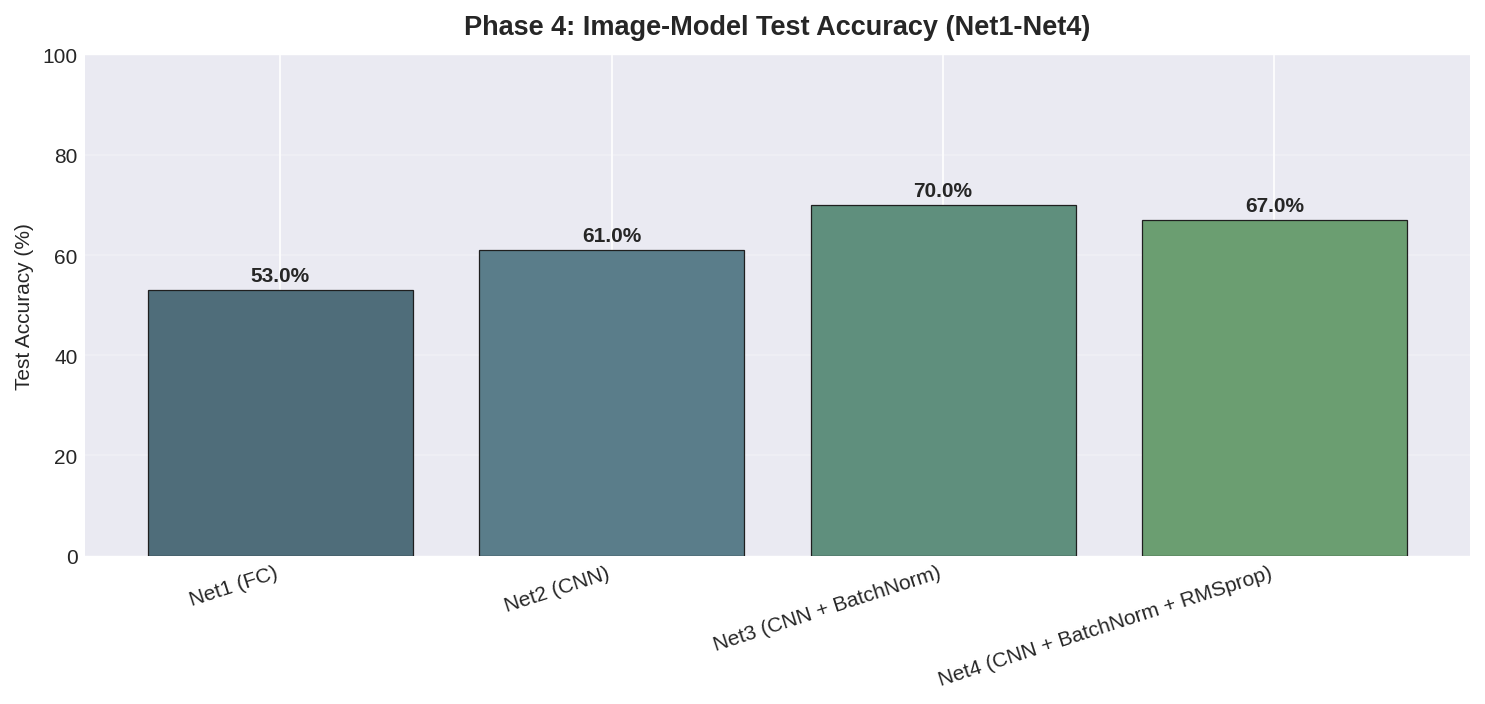
\includegraphics[width=\linewidth]{figures/comparison_image_models_phase4.png}
	\caption{Phase 4 image-model comparison (Net1--Net4).}
	\label{fig:image-phase4}
\end{figure}

\textbf{Net5 (LSTM), 69.0\%.} The sequence model on MFCC features performs strongly and is close to the best CNN result. This indicates that temporal evolution carries useful genre cues.

\textbf{Net6 (LSTM + GAN), 71.0\%.} Net6 is the best overall model and improves Net5 by \textbf{+2.0 points}. The gain is modest but consistent with useful augmentation from synthetic training samples.

\begin{figure}[t]
	\centering
	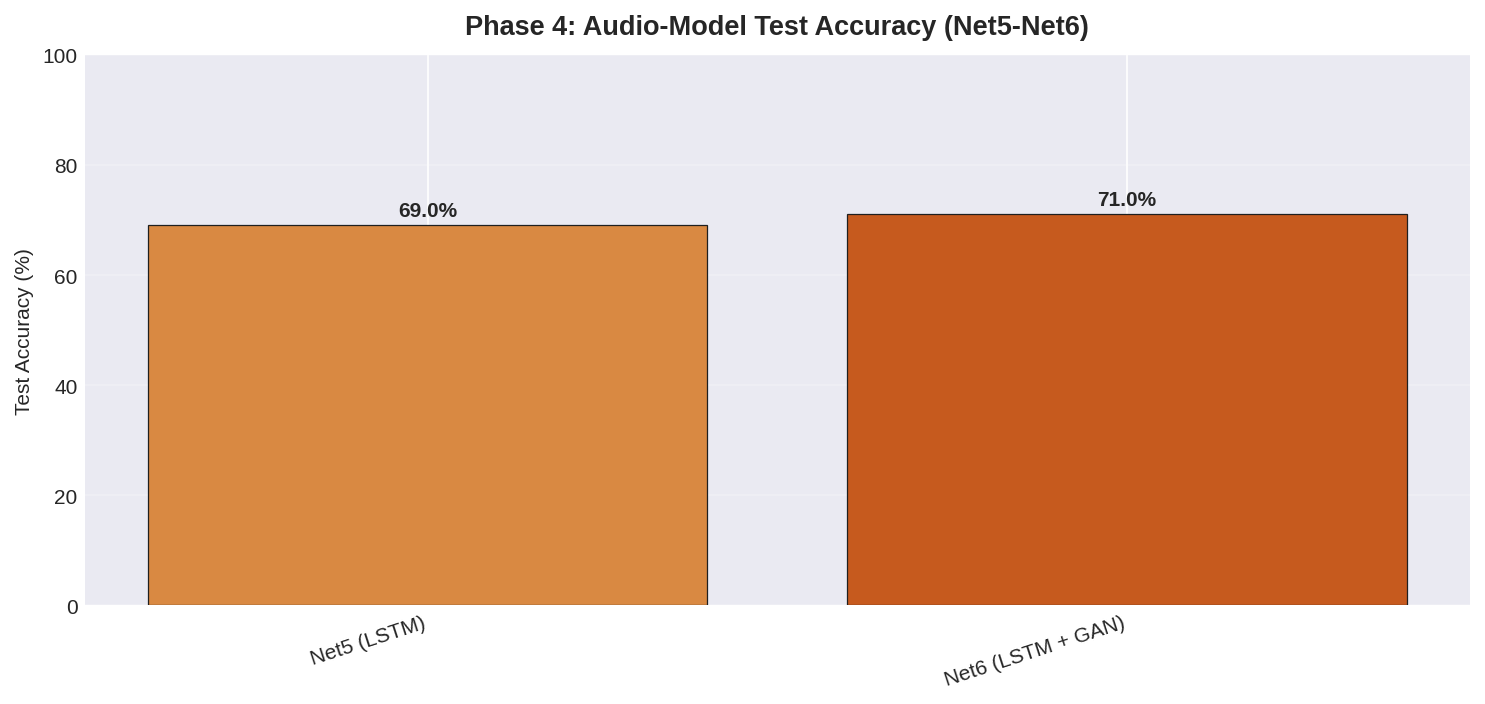
\includegraphics[width=\linewidth]{figures/comparison_audio_models_phase4.png}
	\caption{Phase 4 audio-model comparison (Net5--Net6).}
	\label{fig:audio-phase4}
\end{figure}

\begin{figure}[t]
	\centering
	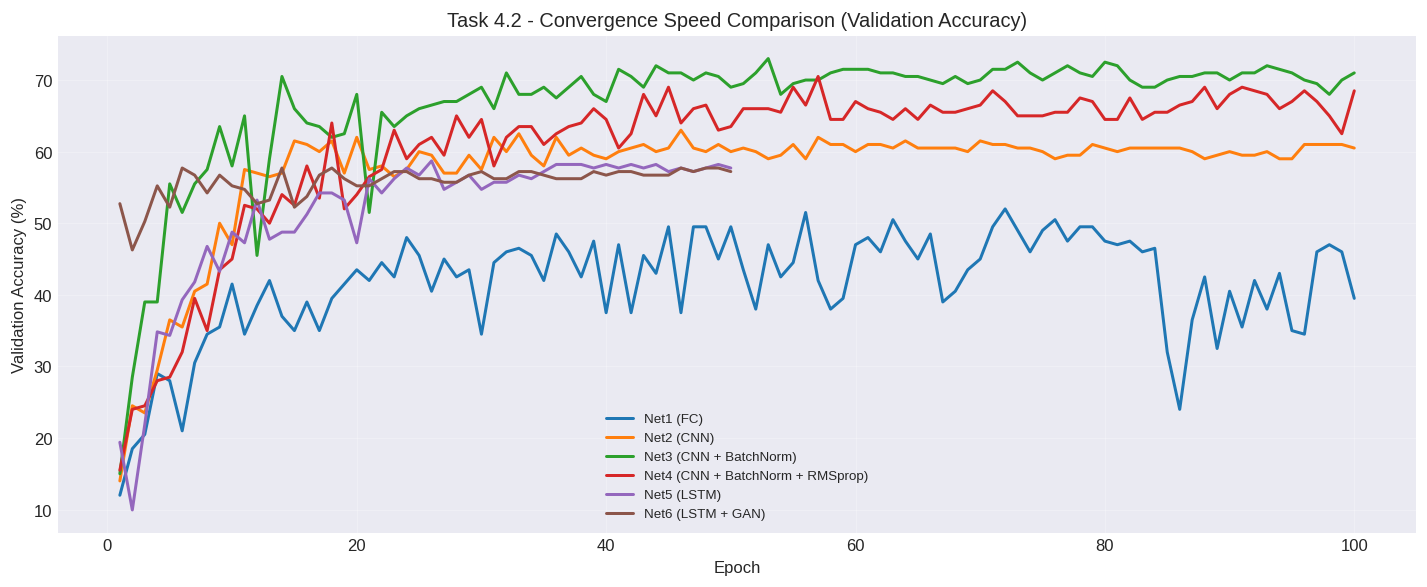
\includegraphics[width=\linewidth]{figures/phase4_convergence_speed.png}
	\caption{Phase 4 validation-accuracy convergence line graph (Task 4.2).}
	\label{fig:phase4-convergence}
\end{figure}

\subsection{Overall Discussion}

Figure~\ref{fig:all-phase4} summarizes the complete ranking across all six models. The top three models are Net6 (71.0\%), Net3 (70.0\%), and Net5 (69.0\%). Mean accuracy is \textbf{70.00\%} for audio models and \textbf{62.75\%} for image models, a \textbf{+7.25-point} advantage for the audio branch on this split.

\begin{figure}[t]
	\centering
	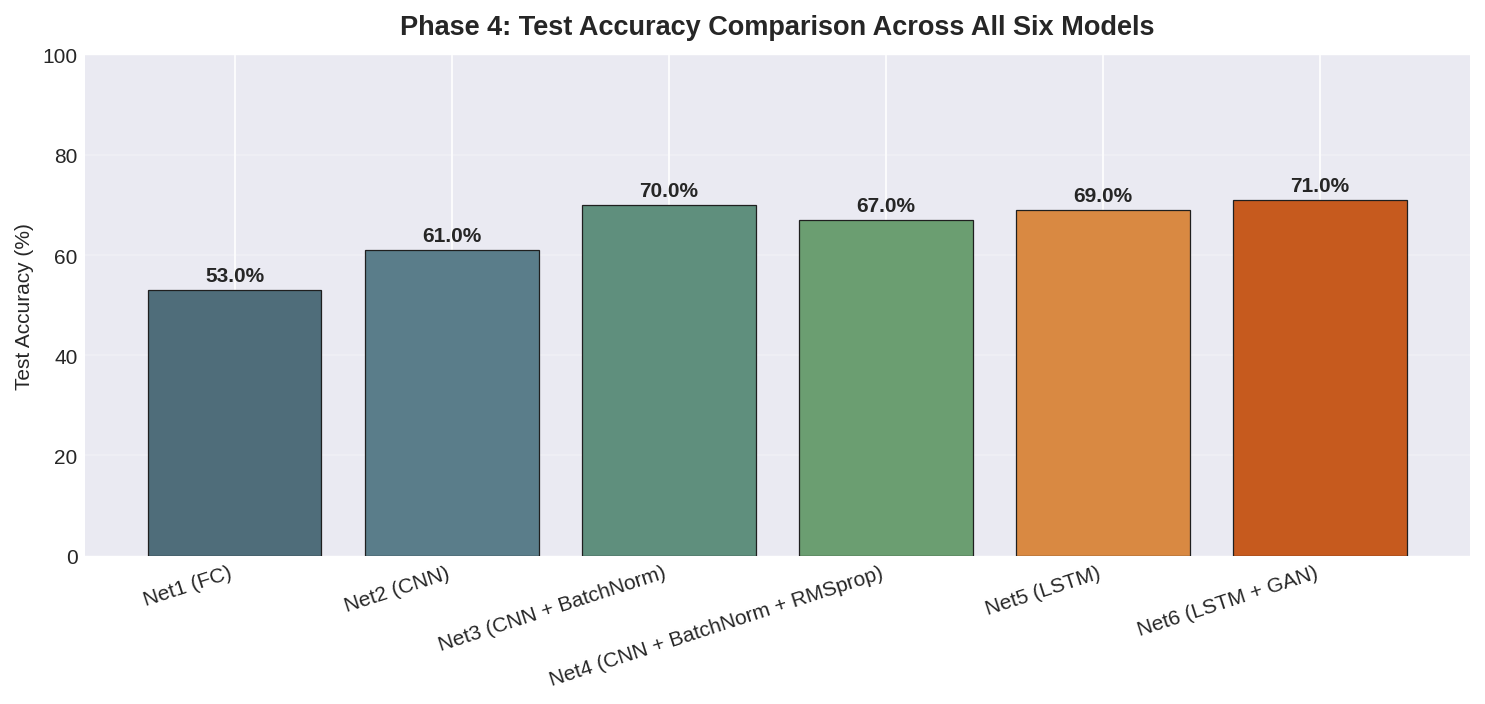
\includegraphics[width=\linewidth]{figures/comparison_all_models_phase4.png}
	\caption{Phase 4 test-accuracy comparison across all six models.}
	\label{fig:all-phase4}
\end{figure}

Genre-level analysis from Phase 4 shows \textbf{jazz} as the easiest class (mean recall 0.95) and \textbf{rock} as the hardest (mean recall 0.30). The most frequent aggregated confusion is \textbf{rock $\rightarrow$ country} (16 errors), which suggests overlap in rhythmic and timbral patterns for these genres in the current feature representation.

\begin{table}[t]
	\centering
	\caption{Complexity and training summary from \texttt{phase4\_model\_complexity.csv} and \texttt{phase4\_training\_time\_comparison.csv}.}
	\label{tab:phase4-complexity-time}
	\scriptsize
	\setlength{\tabcolsep}{3.5pt}
	\resizebox{\columnwidth}{!}{%
	\begin{tabular}{lccc}
		\toprule
		Model & Params (M) & Epoch@90\% Val & Train (s) \\
		\midrule
		N1 (FC) & 87.44 & 24 & 2.23 \\
		N2 (CNN) & 16.13 & 11 & 46.17 \\
		N3 (CNN+BN) & 66.63 & 14 & 63.74 \\
		N4 (CNN+BN+RMSp) & 66.63 & 18 & 63.45 \\
		N5 (LSTM) & 1.51 & 12 & 25.96 \\
		N6 (LSTM+GAN) & 1.51 & 1 & 44.26 \\
		\bottomrule
	\end{tabular}%
	}
\end{table}

\begin{table}[t]
	\centering
	\caption{Top confusion pairs from \texttt{phase4\_aggregated\_confusions.csv}.}
	\label{tab:phase4-top-confusions}
	\scriptsize
	\setlength{\tabcolsep}{3pt}
	\begin{tabular}{@{}lc@{}}
		\toprule
		Confusion Pair & Count \\
		\midrule
		rock $\rightarrow$ country & 16 \\
		blues $\rightarrow$ country & 6 \\
		hiphop $\rightarrow$ reggae & 6 \\
		blues $\rightarrow$ reggae & 6 \\
		metal $\rightarrow$ hiphop & 6 \\
		reggae $\rightarrow$ country & 4 \\
		\bottomrule
	\end{tabular}
\end{table}

\begin{table}[t]
	\centering
	\caption{Genre recall difficulty from \texttt{phase4\_genre\_recall\_difficulty.csv}.}
	\label{tab:phase4-genre-recall}
	\scriptsize
	\setlength{\tabcolsep}{3pt}
	\begin{tabular}{@{}lc@{}}
		\toprule
		Genre & Mean Recall \\
		\midrule
		jazz & 0.95 \\
		classical & 0.92 \\
		hiphop & 0.77 \\
		metal & 0.73 \\
		reggae & 0.63 \\
		disco & 0.63 \\
		pop & 0.60 \\
		blues & 0.50 \\
		country & 0.48 \\
		rock & 0.30 \\
		\bottomrule
	\end{tabular}
\end{table}
\section{Part II: Topic Reflection}
\label{sec:reflection}

\textbf{Selected topic:} \emph{Deep learning for financial time-series forecasting}, with emphasis on diffusion-based generative models.

Financial forecasting is important because prediction quality affects capital allocation, risk control, and market stability. In practice, institutions need more than a single point estimate; they also need uncertainty-aware predictions to support robust decisions during volatile periods.

Current technologies can be grouped into three layers. First, statistical models such as ARIMA, GARCH, and Kalman filtering provide strong interpretability but often struggle with highly nonlinear behavior. Second, discriminative deep models (LSTM, TCN, Transformer) capture long-range temporal dependencies better than many classical approaches~\cite{hochreiter1997lstm}. Third, generative deep models (GANs and diffusion-style models) learn distributions of future trajectories, which is valuable for scenario analysis and risk assessment~\cite{goodfellow2014gan}.

A standard preprocessing step is feature normalization:
\[
x_t^{\mathrm{std}} = \frac{x_t - \mu_t}{\sigma_t}.
\]
For diffusion forecasting, the forward noising process and conditional reverse process are:
\[
q(x_t\mid x_{t-1}) = \mathcal{N}(\sqrt{1-\beta_t}\,x_{t-1},\,\beta_t I),
\]
\[
p_{\theta}(x_{t-1}\mid x_t, c) = \mathcal{N}(\mu_{\theta}(x_t,t,c),\,\sigma_t^2 I),
\]
where $c$ is historical conditional information. A common objective is noise prediction:
\[
\mathcal{L}_{\mathrm{diff}} = \mathbb{E}_{x_0,t,\epsilon}\left[\left\lVert \epsilon - \epsilon_{\theta}(x_t,t,c) \right\rVert_2^2\right],
\quad
x_t = \sqrt{\bar{\alpha}_t}\,x_0 + \sqrt{1-\bar{\alpha}_t}\,\epsilon.
\]

To evaluate forecasting quality, I focus on both absolute and relative errors:
\[
\mathrm{MSE} = \frac{1}{N}\sum_{i=1}^{N}(y_i-\hat{y}_i)^2,
\quad
\mathrm{MAE} = \frac{1}{N}\sum_{i=1}^{N}|y_i-\hat{y}_i|,
\]
\[
\mathrm{SMAPE} = \frac{100\%}{N}\sum_{i=1}^{N}\frac{|y_i-\hat{y}_i|}{(|y_i|+|\hat{y}_i|)/2}.
\]

From this coursework, I can already implement full deep-learning workflows: preprocessing, train/validation/test splitting, CNN/LSTM training, and rigorous metric-based comparison. I can also present model behavior through convergence plots and error analysis.

However, I cannot yet implement a production-grade financial diffusion system with reliable uncertainty calibration and robust trading backtests. The main technical barriers are preventing temporal leakage, tuning diffusion schedules efficiently, handling regime shifts, and aligning ML metrics with economic utility under transaction costs.

The positive impact of current deep learning technology is better nonlinear modelling, stronger scenario generation, and potentially improved risk-aware planning. The negative impact includes limited interpretability, overfitting risk under non-stationarity, high computational cost, and possible misuse in highly leveraged or opaque decision pipelines.

My future vision is to build hybrid and responsible systems that combine sequence encoders with conditional diffusion scenario generators, then optimize decisions under explicit risk constraints. Beyond prediction error, I would track decision quality using risk-adjusted metrics such as:
\[
\mathrm{Sharpe} = \frac{\mathbb{E}[R]-R_f}{\sigma(R)}.
\]
This aligns evaluation with risk-aware decision making in quantitative finance.
The long-term goal is not only accurate forecasting, but trustworthy, interpretable, and risk-aware AI for finance.

{
    \small
    \bibliographystyle{ieeenat_fullname}
    \bibliography{main}
}

\end{document}
